\section{Transfer to marked Jordan quadrilaterals}\label{sec:jordan}

Throughout Sections~\ref{sec:jordan}--\ref{sec:chordal}, fix
$1\le q<4$ and write
\[
 d=\sqrt q=2\cos\lambda,\qquad \rho=\lambda/\pi,
 \qquad h=1-2\rho\in[1/3,1).
\]
The four-change calculation of Section~\ref{sec:fourchange}, whose
holomorphicity hypothesis is supplied in Section~\ref{sec:holomorphic},
gives the functions
\begin{equation}\label{jordan:functions}
 f(\chi)=\frac{I_C(\chi)}{I_B(\chi)+I_C(\chi)},\qquad
 g(\chi)=\frac{f(\chi)}{f(\chi)+d(1-f(\chi))},
 \quad 0<\chi<1,
\end{equation}
where
\begin{align*}
 I_B(\chi)&=\int_\chi^1
 u^{\rho-1}(u-\chi)^{\rho-1}(1-u)^{1-3\rho}\,du,
 \\
 I_C(\chi)&=\int_1^\infty
 u^{\rho-1}(u-\chi)^{\rho-1}(u-1)^{1-3\rho}\,du.
\end{align*}
The first function is the probability in the open-cap normalization;
the second is the probability of an \emph{actual open path} between the
two separately wired intervals.  Wiring changes component weights; it
does not supply an open path between different intervals.

\begin{proposition}[Jordan-quad transfer]\label{jordan:transfer}
Consider the marked, uniformly convergent square lattice polygon
approximations $(D_n;a_n,b_n,c_n,d_n)$ to a bounded Jordan quadrilateral
$(D;a,b,c,d)$ in the four-mark sense of Subsection~\ref{intro:crossings}.
Keep every edge of the polygon graph random, and separately wire the two closed arcs $a_nb_n$ and
$c_nd_n$, with no other primal identifications.  If
$\psi:D\to\mathbb H$ sends $(a,c,d)$ to $(0,1,\infty)$ and
$\chi=\psi(b)$, the probability of an actual open path between these
arcs tends to $g(\chi)$.
\end{proposition}

\begin{proof}
First consider a fixed rational orthogonal polygon in tile coordinates.
The deterministic caps of Section~\ref{sec:preliminaries} contribute
one or two additional loops according to the pairing.  Their weight
ratio is exactly the factor $d$ in \eqref{jordan:functions}, so the
four-change formula gives $g$.  If its designated color lies on the
dual grid, translate the complete tile domain, switches, and caps by
one tile step.  This preserves its loop law and makes that color the
prescribed primal grid, at a geometric cost $O(\delta_n)$.  Consequently
there are suitable approximations of every fixed test polygon on the
\emph{same} lattice as the target graph.

Choose a plane Schoenflies homeomorphism taking $\overline D$ to the
unit square, with the two electrodes on the left and right sides.
Uniform marked boundary convergence and winding number imply the
following strict inclusions for all sufficiently large $n$: $D_n$
contains every closed inset square and is contained in every prescribed
neighborhood of the square in these coordinates; its four marked arcs
are close to their corresponding sides.  Fix $\varepsilon>0$.
In physical coordinates polygonize the pullbacks of
\[
 [\varepsilon,1-\varepsilon]\times[-\varepsilon,1+\varepsilon]
 \quad\hbox{and}\quad
 [-\varepsilon,1+\varepsilon]\times[\varepsilon,1-\varepsilon].
\]
Call these the easier and harder test quads, respectively, and put
their electrodes on the nearly vertical sides.  Take the polygonization
error in Schoenflies coordinates smaller than $\varepsilon/10$, with
marks in flat side interiors, and retain this margin after all tile
translations.  Such simple rational orthogonal polygonizations exist:
first use radial shrinking in a Carath\'eodory disk parametrization to
obtain an analytic Jordan approximation, then a fine simple polygon;
replace each segment by a rectangular staircase inside its own thin
corridor and join adjacent staircases in disjoint small vertex
neighborhoods.  The marks can be placed in order in side interiors.
These constructions give marked uniform convergence as
$\varepsilon\downarrow0$.

\begin{figure}[tb]
\centering
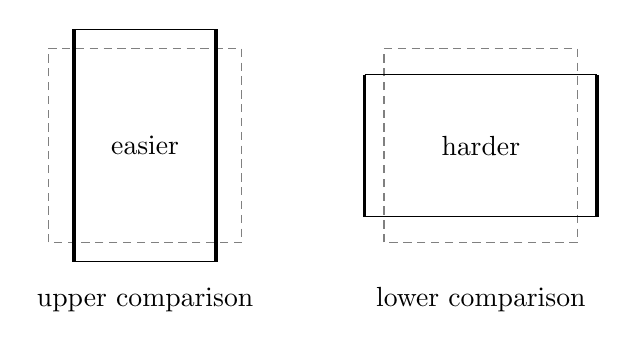
\begin{tikzpicture}[scale=.82]
 \begin{scope}
  \draw[densely dashed,gray] (0,0) rectangle (3,3);
  \draw (0.4,-.3) -- (2.6,-.3) (0.4,3.3) -- (2.6,3.3);
  \draw[very thick] (0.4,-.3) -- (0.4,3.3)
                   (2.6,-.3) -- (2.6,3.3);
  \node at (1.5,1.5) {easier};
  \node[below] at (1.5,-.55) {upper comparison};
 \end{scope}
 \begin{scope}[xshift=5.2cm]
  \draw[densely dashed,gray] (0,0) rectangle (3,3);
  \draw (-.3,.4) -- (3.3,.4) (-.3,2.6) -- (3.3,2.6);
  \draw[very thick] (-.3,.4) -- (-.3,2.6)
                   (3.3,.4) -- (3.3,2.6);
  \node at (1.5,1.5) {harder};
  \node[below] at (1.5,-.55) {lower comparison};
 \end{scope}
\end{tikzpicture}
\caption{The Jordan-quad comparison in Schoenflies coordinates.
The dashed square is the limiting target; thick sides are separately
wired electrodes.  The easier quad extends beyond the free sides and
ends inside the target's electrode sides.  The harder quad has the
opposite inclusions.  Physical test polygons retain strict margins
after pullback and lattice approximation.}
\label{jordan:sandwich-figure}
\end{figure}

For the upper bound, restrict both laws to their common primal edges
in the easier quad.  Any target edge outside this common graph can
attach to it only on its two electrode sides: the easier horizontal
sides lie strictly outside the target.  Outside pieces cannot join
the two electrode sides, even through a target wire block, because
the substantial intervening strip lies wholly inside the easier quad
and the two target wire blocks lie in separate exterior zones.
Thus the target's induced boundary partition on the common graph is
weaker than separate wiring of the easier electrodes.  Domain Markov
and FK monotonicity give a coupling in which the easier common-edge
configuration dominates the target's.  Every actual target crossing
contains a common-edge crossing of the easier electrodes.  Indeed,
follow it from the initial exterior zone to the opposite zone, taking
its last exit from the first and first entry into the second; its
intermediate edges must belong to the common graph.  There is no
escape through the distant horizontal sides.

For the lower bound interchange the roles using the harder quad.
Its exterior pieces can attach to the target only on the designated
target arcs, and cannot link opposite sides outside the common graph.
Here it matters that the target contains \emph{all} lattice edges in
its closure, and that both graphs use exactly the same primal grid.
The target wires therefore dominate the induced harder-quad
partition.  Every harder crossing contains an actual shared-edge
piece joining the two target arcs.  This proves the lower comparison.
All transitions occur at ordinary graph vertices; shrinking lattice
edges have uniformly shrinking diameter in Schoenflies coordinates,
so the strict margins justify the discrete versions of the statements.

The conformal cross-ratios of the two test quads tend to $\chi$.
Indeed uniformly convergent parametrizations of Jordan curves imply
uniform local connectedness of their boundaries: points close in the
image have parameters close in the circular order, except for the
identified endpoints, because the limiting parametrization is an
embedding.  Kernel convergence and boundary extension of normalized
Riemann maps then give marked conformal convergence
\cite{Pommerenke1992}.  Since $g$ is continuous on $(0,1)$, let first
$n\to\infty$ and then $\varepsilon\downarrow0$ in the two comparisons.
\end{proof}

\begin{corollary}[The prescribed bond-percolation crossing]\label{jordan:cardy}
At $q=1$, with every edge, including every boundary edge, sampled
independently with probability $1/2$ and with no wiring, the probability
of the event $C_n$ defined in Subsection~\ref{intro:crossings} tends to
\[
 \frac{\displaystyle\int_0^\chi [t(1-t)]^{-2/3}\,dt}
      {\displaystyle\int_0^1 [t(1-t)]^{-2/3}\,dt}.
\]
\end{corollary}
\begin{proof}
For $q=1$ the boundary partition does not change the edge law, and
$d=1$ gives $g=f$.  The $\rho=1/3$ specialization of the four-change
integral calculation is precisely the displayed expression.  The
comparison in Proposition~\ref{jordan:transfer} concerned actual edge
paths throughout, so no external wire is counted as a crossing and
no interface-event continuity assertion is needed.
\end{proof}

\section{Alternating tests after exploration}\label{sec:movingtests}

The Jordan result alone does not apply to a domain cut out by a random
exploration.  We prove the needed extension directly under the
original lattice law.  Conditional errors at exceptional histories
will be controlled by an \emph{averaged} six-arm estimate.

\subsection{Geometry and conditional laws}

\begin{lemma}[A compatible simple drawing]\label{moving:drawing}
The prescribed polygon graph and its Dobrushin strand admit a tile
and collar representation in a Jordan polygon $V_n$ such that:
\begin{enumerate}[label=(\roman*)]
\item $V_n$ has the same marked uniform Jordan limit as $D_n$;
\item the rounded strand is simple, visits the same ordered local
pieces as the prescribed medial strand, and is at curve distance
$O(\delta_n)$ from it;
\item at every switch-revealing stop, the remaining domain is a simple
slit disk.  Under deterministic cap closure its unrevealed edges have
the original conditional FK law, with known open edges contracted
and known closed edges deleted;
\item primal and dual banks of the prefix have physical access to
their corresponding known edges and wire vertices within
$O(\delta_n)$.  Every completion of the unknown edges embeds its
actual paths in the slit disk without crossing the past.
\end{enumerate}
The construction can use identical domains and caps away from an
interval where two additional boundary changes are inserted.
\end{lemma}

\begin{proof}
Make one tile for each edge of the polygon graph, including boundary
edges.  Glue the four triangles directed toward each interior square
center.  The exterior triangle of a boundary edge is a separate tab,
with its own outer dual vertex; do not glue different exterior tabs
along their radial sides.  Each primal boundary vertex retains all
its interior incidences.  Flatten the exterior tabs toward their
bases, to less than half their original height, and add a still
thinner Jordan collar.  The tabs are then disjoint except at their
prescribed vertices.  All changes lie within $O(\delta_n)$ of the
original boundary, and tracing the tabs and collar along the original
parametrization proves (i).

Draw the switches and boundary caps as disjoint arcs.  A local wire
can be drawn behind its cap in the collar.  The unmatched ports
continue to the marked outer-boundary points.  The finite choices
inside each tile and the collar can be made deterministically.
At a wired boundary edge, capping its outer dual vertex joins the
inside ports in the same way for either switch state.  Declaring that
edge open for the drawing merely substitutes a cap-sized detour and
possibly deletes a microscopic loop.  On the free side, the cap
around a primal vertex is exactly the turn beside the dual wired
arc.  Inside the polygon, glued half-segments give the specified
medial edges and their quarter-turn pairings.  Match corresponding
ordered pieces in the two drawings.  Each substituted piece lies in
boundedly many neighboring tiles, so simultaneous parametrizations
have distance $O(\delta_n)$.  Zero-length pieces are handled by limits
of increasing reparametrizations.  This also covers a midpoint visited
with both prescribed pairings and proves (ii).

The tile/cap Euler identity gives exactly the conditional FK law
asserted in (iii).  On a queried primal-open tile the adjacent primal
corners are joined by its actual edge; on a queried closed turn the
bank stays at one primal corner.  Along a cap it stays at one vertex
or uses neighbors already belonging to that wire interval.  Thus the
bank is a known chain attached to the appropriate original interval,
and every queried primal-open edge accesses this bank within one tile.
The same statement holds for dual edges.  Designated outer vertices
access their arcs through the collar.  These are physical accesses,
not additional identifications.  They prove (iv), also when the last
begun tile is revealed in full.  Projecting back to the usual primal
or dual lattice moves points by $O(\delta_n)$ and duplicates no edge;
separate virtual copies of a vertex may become one physical vertex.
\end{proof}

In a four-open-change experiment, deterministic closure with separate
wires of one color differs by a density depending only on the two
pairing outcomes.  This density and its reciprocal are bounded by
constants depending on $q$.  At a switch-revealing stopping time the
odds change is still exactly
\begin{equation}\label{moving:odds}
 p\longmapsto \frac{p}{p+d(1-p)}.
\end{equation}
One obtains this by conditioning the \emph{full} finite-sample density,
not by postulating a Markov property for a limiting curve.  Consequently
conditional rare-event probabilities in a deterministic-cap law can
be averaged under open-cap histories at a bounded multiplicative cost.

\begin{lemma}[Small-interval behavior]\label{moving:asymptotic}
For $f$ in \eqref{jordan:functions},
\[
 f(1-\chi)=1-f(\chi),\qquad
 f(\chi)=c_q\chi^h(1+o(1))\quad(\chi\downarrow0),
 \qquad c_q>0.
\]
\end{lemma}
\begin{proof}
The substitutions $u^{-1}$ in $I_C$ and
$u=1-(1-\chi)t$ in $I_B$, followed by the Euler transformation of
the beta integral, give
\[
 I_B(\chi)=\left(\frac{1-\chi}{\chi}\right)^h I_C(1-\chi).
\]
Both $I_C(0)$ and $I_C(1-)$ are finite and strictly positive: at the
possible singularity $u=1$, the latter integrand has exponent
$-2\rho>-1$, while the integrand at infinity has exponent
$-1-\rho<-1$.  Substitution into \eqref{jordan:functions} proves both
claims, with $c_q=I_C(0)/I_C(1-)$.
\end{proof}

\begin{theorem}[Moving four-change test]\label{moving:slit}
Let a four-change strand in $V_n$ be stopped before completing its
strand, revealing only the switches it has encountered.  Let $U_n$
be its remaining simple slit disk, with the tip as the new starting
mark.  Consider histories for which a fixed basepoint has a fixed
positive disk in $U_n$, and the four prime-end marks in a disk chart
normalized at that basepoint remain mutually separated by a fixed
positive amount.  Then, on these histories,
\begin{equation}\label{moving:limit}
 \mathbb P_{\mathrm{open}}(E_{\mathrm P}\mid\mathcal F_n)
       -f(\chi_{U_n})\ \longrightarrow\ 0
 \quad\hbox{in probability}.
\end{equation}
Here $E_{\mathrm P}$ is the primal pairing event, equivalently the
actual bridge event after separate primal closure, and $\chi_{U_n}$
is its current ordered cross-ratio.  The assertion holds for arbitrary
mesh-dependent stopping rules satisfying this localization.
\end{theorem}

We supply the proof in several steps.  Every annulus used below lies
a fixed positive distance inside the original domain before its mesh
limit is taken.  The inputs are the bulk passage estimate of
Section~\ref{sec:preliminaries}, the vanishing full-lattice one-arm
bound with wired rims, and the six-arm estimate
\begin{equation}\label{moving:sixarm}
 \mathbb P(A_6(r,R))\le C(r/R)^{2+c_0},\qquad c_0>0,
\end{equation}
for the critical square-lattice FK law with this fixed $q<4$
\cite[Corollary~6.7]{DMT2021Fractal}.  An outer buffer and the bulk
boundary-condition comparison transfer this estimate from the
infinite-plane law to the original finite law.  Bounded open-cap
reweightings are harmless.  No six-arm estimate conditioned on an
arbitrary explored maze is asserted.

\begin{lemma}[Physical paths and chart oscillation]\label{moving:chart-modulus}
Let $u_n$ be the horizontal coordinate of the conformal rectangle
map of $U_n$, with the designated primal arcs at $0$ and $1$.
Under the localization in Theorem~\ref{moving:slit}, there is a common
modulus tending to zero for the oscillation of $u_n$ on a connected
path of vanishing physical diameter, including paths with accesses
to the prime boundary.  Consequently, for $\beta>0$, a possible
primal path starting in $\beta\le u_n\le1-\beta$ cannot reach a known
primal-open edge or a primal electrode inside a sufficiently small
physical ball.  ``Possible'' means that all still unknown primal
edges are filled open, before any external wire jump is permitted.
\end{lemma}
\begin{proof}
Away from the normalizing point, a connected set in a ball of radius
$r$ is hit before domain exit by Brownian motion from that point
with probability tending uniformly to zero as $r\downarrow0$.
Comparison with a fixed enclosing Euclidean annulus gives this
bound.  In the normalized disk, a connected set of a fixed positive
diameter has hitting probability bounded below; this follows, for
example, by a crosscut between separated angular sectors and the
Beurling estimate.  The rectangle maps of the disk form a compact
family because the four marks remain separated.  Thus a small
physical continuum cannot have a macroscopic rectangle-coordinate
oscillation.  Near the basepoint use interior distortion instead.
Endpoint accesses follow by interior approximation.

By Lemma~\ref{moving:drawing}, every known primal-open edge and fixed
primal wire attachment accesses $u_n=0$ or $1$ within
$O(\delta_n)$.  A short possible connection from the central band to
one of them would contradict the just-proved modulus.  Small buffers
in the band absorb individual tile errors.  In particular the two
opposite designated intervals have not already met through the
revealed bank under the stated nondegeneracy.
\end{proof}

\begin{lemma}[Deletion and protected-ball costs]\label{moving:deletion}
Fix a history and use separate deterministic primal closure.
Deleting a set of still random edges changes the actual crossing
probability by at most the conditional probability that an endpoint
of a deleted edge reaches a wire interval by an actual open path,
allowing one initial test step over the deleted edge.
For a central-band set contained in a ball of radius $r$, this cost
is bounded by a quantity tending to zero as $r\downarrow0$,
uniformly in the history and center, provided its required outer
radius is fixed and the mesh is sufficiently small.  The same holds
for any fixed finite number of such balls.
\end{lemma}
\begin{proof}
Couple the deleted and original laws monotonically.  Explore the
actual open clusters from all deletion endpoints in the stronger
configuration, revealing the corresponding edges in both laws.
FK partition monotonicity persists at every step.  After the clusters
are enclosed by their closed cuts, the conditional laws outside
agree and can be coupled identically.  If no explored cluster reaches
a wire interval, the crossing decision is unchanged.  This proves
the first assertion, including contact with a wire along a known bank.

Choose the fixed outer radius small enough for
Lemma~\ref{moving:chart-modulus}.  Every component of possible edges
inside this ball that meets the central-band set has no accessible
wire or known primal-open attachment.  Its uncertain boundary
connections can occur only at the ball rim.  Project to the physical
lattice, fill missing edges, and wire that rim.  Splitting physical
vertex copies only weakens the original induced partition.  The
full-lattice wired-rim law therefore dominates every relevant actual
arm simultaneously.  Cropping the ball slightly absorbs tile errors.
Its one-arm probability from radius $r$ to the fixed outer radius
tends to zero: buffered dual circuits from RSW block such an arm.
A finite union bound gives the last assertion.
\end{proof}

\subsection{A directed obstacle away from possible connections}

Fix a small trimming parameter $a_*>0$ and then
$0<\beta<a_*/20$.  A primal vertex is a \emph{candidate} if its chart
coordinate lies in $[\beta,1-\beta]$ and it has a possible connection
to an electrode.  Each candidate supplies a possible arm to a fixed
positive physical distance, by Lemma~\ref{moving:chart-modulus}.

\begin{lemma}[Flagged cells and their cost]\label{moving:flags}
In a fixed bulk block let $\pi$ be a simple known primal bank path.
Choose fixed scales $\ell\ll R_1$, away from its endpoints and the
original boundary.  Flag a deterministic grid cell of side $\ell$
if, in its annulus from $100\ell$ to $R_1$, the prefix already supplies
four cyclically alternating actual arms, its two primal arms being
known wired bank paths.  If a candidate within $O(\ell)$ of this cell
actually connects to an electrode, then six actual alternating arms
occur in a cropped annulus from $200\ell$ to $R_1/2$.
For a bounded region covered by the deterministic cells, the averaged
conditional attachment cost of all flagged cells is at most
\begin{equation}\label{moving:flag-sum}
 C\ell^{-2}(\ell/R_1)^{2+c_0}=O_{R_1}(\ell^{c_0}).
\end{equation}
The statement remains valid with one initial test step and with the
bounded cap changes in \eqref{moving:odds}.
\end{lemma}
\begin{proof}
The extra actual primal arm cannot make a lateral connection to
either known primal leg inside the wider annulus, even in the
all-unknown-primal-open completion, by
Lemma~\ref{moving:chart-modulus}.  On the side containing the extra
arm it is bracketed by the two known primal legs.  A planar crossing
alternative in each intervening strip supplies a dual radial
separator.  The original dual separator on the other side remains.
After cropping at both rims, these three primal and three dual arms
are disjoint and alternate.

For precision, thicken actual paths to their tile color territories.
An open transversal between two primal territories would give an
actual lateral bridge, with an error of at most one tile.  Its absence
forces a dual territorial radial crossing in the intervening
topological rectangle, which shadows a dual edge path in the cropped
annulus.  If the no-bridge test is made after every unknown primal
edge is opened, every dual separator so obtained consists of known
closed tiles.  Thus the four old legs and the separators used in
this argument are actual original edges; no auxiliary boundary
condition manufactures them.

Apply \eqref{moving:sixarm} in the original full-sample law to each
cell of the deterministic grid, then sum over $O(\ell^{-2})$ cells.
The center may have been selected by the past because the sum was
taken over the entire deterministic grid.  Bounded cap densities
control the averaged conditional probabilities under either history
law.  Markov's inequality now makes the conditional flagged-cell
cost small outside a set of histories of small probability.  This
is an annealed-to-conditional argument, with $R_1$ and all comparison
constants fixed before $\ell\downarrow0$.
\end{proof}

\begin{lemma}[Directed obstacle]\label{moving:obstacle}
After removing histories of arbitrarily small probability and allowing
an arbitrarily small conditional deletion cost, there is a Jordan
polygon $H$ containing the basepoint, selected from a finite list at
each fixed accuracy, with the following properties.
Its boundary follows the original boundary and explored prefix to
that accuracy; away from finitely many protected balls and flagged
cells it has fixed positive clearance from all central candidates.
As the accuracies decrease, $H$ and $U_n$ have the same pointed kernel
limits.  Artificial marks in $H$ may be chosen with disk angles
arbitrarily close to the corresponding angles in $U_n$.
\end{lemma}
\begin{proof}
We give the construction and its scale order.  Retain only prefix
excursions reaching depth $r$ from the limiting Jordan boundary,
including each complete segment between successive visits to depth
$h_b\ll r$ and the last incomplete segment if present.  Their number
is tight, uniformly in small $h_b$, because each visits one of a fixed
finite family of bulk annuli at depth $r/2$.  First bound this number,
then choose $h_b$ small.  Join their boundary-near endpoints to the
exterior of a slightly larger polygon through protected balls of
radius $O(h_b)$.  Lemma~\ref{moving:deletion} controls central
attachments in these finitely many balls.  No boundary arm exponent
for the rough Jordan curve is needed.

Break the retained excursions into blocks of diameter at most
$\epsilon\ll h_b$, each contained with margin in a bulk square $S$
of side $10\epsilon$.  Successive displacement thresholds and the
bulk passage estimate make the number of blocks tight.  After fixing
a block-count cutoff, snap its endpoints to a much finer deterministic
grid and protect them by balls of radius $e\ll\epsilon$.  The actual
known primal bank gives a path between the true endpoints in $S$;
loop erasure gives a simple path $\pi$, possibly trivial.  Take
\[
 \ell\ll R_1\ll e,
\]
so all flag annuli are bulk annuli.  Declare forbidden every closed
$\ell$-cell within $3\ell$ of a candidate, except flagged cells and
cells in enlarged endpoint protections.

There is a connector between the protected endpoints avoiding all
forbidden cells.  Otherwise planar cell separation gives a polygonal
circuit through a chain of touching forbidden cells and possibly the
exterior of $S$, separating the two endpoints.  It can be chosen
away from their protection balls and within a cell-sized error of
the cell chain.  Choose a candidate witness in each cell.  Two
successive witnesses can be joined avoiding $\pi$ inside a disk of
radius $O(R_1)$.  If they could not, a proper crosscut of the simple
path $\pi$ would separate them in a circle of radius between
$4R_1$ and $6R_1$.  Its full-path endpoints lie outside because the
cell is away from endpoint protections.  The crosscut passes within
$O(\ell)$ of the witness segment.  The two witnesses have possible
arms to that circle, on opposite sides of $\pi$, and cannot connect
locally to $\pi$ by Lemma~\ref{moving:chart-modulus}.  The two known
radial legs of $\pi$ and the two possible arms consequently interlace.
In each intervening strip the optimistic no-bridge test supplies a
\emph{known} dual radial separator, as in the proof of
Lemma~\ref{moving:flags}.  The cell is therefore flagged, a
contradiction.

Push the separating circuit through the witness points and these
avoiding joins.  Its displacement is $O(R_1)$, smaller than its
distance from the endpoints, so its winding distinction is preserved.
Along the exterior of $S$ avoidance is automatic because $\pi$ has
an interior margin.  We have obtained a separating circuit disjoint
from $\pi$, which is impossible.  Overlapping endpoint protections
or a trivial $\pi$ are handled by a connector within their union.

Select one polygonal connector for each allowed finite grid pattern.
Their union and the protected exterior attachments form an obstacle
$K$ attached to the complement of the larger polygon.  The connectors
need not form one simple curve.  They stay close to the retained
prefix, and every omitted prefix piece is boundary-near; conversely
the entire prefix is approached by this obstacle or the outer wall.
Within distance $\ell/2$ of $K$, candidates occur only in flagged or
protected error regions.  The basepoint component of the complement
is simply connected, because each obstacle component is attached to
the exterior.  It is a fixed polygonal domain, possibly with slits
and pinches.  An interior radial approximation in its Riemann map,
followed by a polygonal perturbation, gives a Jordan domain $H$ whose
boundary is within $\ell/10$ of the obstacle or outer wall.
The outer wall was chosen much farther than $\ell$ from the original
graph.  Hence the asserted clearance holds.  Every choice is from a
finite list at fixed scales and count cutoffs.

Normalize maps of $H$ and $U_n$ at the same basepoint, and transfer
marks by finite-grid approximations to their disk angles.  On a
Hausdorff subsequence of the original boundary and prefix, every
compact path in the limiting basepoint component eventually belongs
to both constructions, while every limiting boundary point is
approached by complements of both.  Thus their pointed kernels agree,
and their normalized interior charts have the same limit.  This is
an interior statement; no locally connected boundary for the
limiting slit domain is asserted.  The fixed basepoint margin and
separation of the marks persist throughout.
\end{proof}

\subsection{Alignment of the comparison charts}

\begin{proof}[Proof of Theorem~\ref{moving:slit}]
It suffices to prove an upper bound for the primal connection under
separate deterministic primal closure.  Interchanging the colors
and using the other deterministic closure gives the complementary
upper bound; \eqref{moving:odds} then yields the open-cap limit.

Use Lemma~\ref{moving:obstacle}, and write $u$ and $v$ for the rectangle
abscissas in $U_n$ and $H$.  Test on the Jordan subquad of $H$ between
$v=a_*$ and $v=1-a_*$, with these sides separately wired.  At fixed
accuracy there are finitely many such quads; approximate each on the
original color grid by the polygon construction of
Proposition~\ref{jordan:transfer}.  Their limiting crossing
probabilities differ from $g(\chi_{U_n})$ by arbitrarily small
trimming, chart-angle, and kernel errors, uniformly under the
nondegeneracy assumptions.

We justify comparison on shared edges.  Take a fine finite grid of
abscissa bins in the central part of $(0,1)$, with width much smaller
than both $\beta$ and $a_*$.  In each bin choose a nearby vertical
fiber for each chart.  Its central part is a compact internal curve
and is matched in the other chart by kernel convergence.  Its two
remaining tails can be confined to balls of vanishing radius,
with matched centers.  Here is the required length--area argument.
Remove small fractions of rectangle height at top and bottom.
For each fixed fraction, inverse maps and derivatives converge on
the compact retained rectangles.  Let that fraction decrease slowly.
For a bin $I$ and a deleted height interval $J$, Cauchy--Schwarz gives
\[
 \int_I\!\operatorname{length}\bigl(\Phi(\{x\}\times J)\bigr)\,dx
 \le (|I||J|)^{1/2}
       \left(\int_{I\times J}|\Phi'(z)|^2\,dA(z)\right)^{1/2},
\]
where $\Phi$ is the inverse rectangle map.  The last integral is
bounded by the common physical area bound.  Choose levels in each
bin controlling the tails of both charts.  Their initial endpoints
match on the retained compact pieces, so matched small endpoint
balls contain all four tails.  This argument does not require
uniform local connectedness of the explored boundaries.  Tile errors
are absorbed by decreasing the fractions slowly enough.
Lemma~\ref{moving:deletion} controls the conditional attachment cost
of these finitely many endpoint balls.

Delete still unknown edges touching a slightly narrower band,
initially $3\beta\le u\le1-3\beta$, if their endpoints fail containment
in $H$ with a sufficiently small fixed fraction of the clearance
$\ell$, or if their two abscissas differ by more than $a_*/10$.
These deletions have negligible conditional crossing cost.  To see
this, suppose an endpoint of such an edge reaches an electrode by
an actual path, allowing the initial test step.  Paths meeting a
flagged cell, protection ball, or fiber-endpoint ball while centrally
located already have negligible total cost.  For every other path,
trace it inward from the electrode after its last entry into the
broader band $2\beta\le u\le1-2\beta$.  It crosses a comparison
$u$-fiber on its main internal piece, giving an anchor in $H$ with
nearly equal abscissas.  It cannot subsequently leave $H$, since its
central vertices are candidates and the wall has clearance from
them.  Each later crossing of either chart's comparison fiber is
again on its main piece.  If $v$ drifted by more than a few bin
widths from $u$, it would cross a $v$-fiber in a nonmatching $u$-bin,
a contradiction.  The endpoint therefore has neither proposed
defect.  Vertices without a possible electrode connection can be
discarded at no crossing cost.  Smaller nested bands and clearance
constants accommodate complete edge segments and physical-grid
projection.

Now keep the surviving uncertain edges in
$4\beta\le u\le1-4\beta$ that also belong to the trimmed test graph.
A nonshared original piece can attach to these only on a designated
side of the test quad: clearance excludes its free horizontal sides,
and the abscissa buffers exclude an attachment from a noncentral
piece.  No nonshared piece, even with history wires, connects the
two designated sides.  Such a traversal must pass through the middle
shared strip by chart matching, while all identifications lie in the
two separate groups near $u=0,1$.  After matching physical vertices,
the induced original partition is thus dominated by the test law's
separate wiring.  Every modified original actual crossing contains
a shared crossing between the test sides, by taking its traversal
from the first exterior group to the second.  Domain Markov and
partition monotonicity give the desired test upper bound.

For completeness, the construction has the following quantifiers.
If convergence in probability failed with fixed error and probability,
choose first $a_*$ small, then $\beta$ and fiber precision smaller.
Choose obstacle accuracies tending to zero, with, at each stage,
a deep-excursion cutoff, boundary protection radius $h_b$, block
sizes and count cutoffs, endpoint protections $e$, the intermediate
radius $R_1$, and finally the flag scale $\ell$.  The conditional
protection costs and the averaged flag cost
\eqref{moving:flag-sum} are made small in that order.  For each fixed
stage choose the lattice mesh small enough for every geometric margin
and each of the finitely many Jordan test limits.  Select failing
histories outside all exceptional sets, and pass to a common kernel
subsequence.  The fiber argument and additional deletions along this
subsequence have uniform conditional error by
Lemma~\ref{moving:deletion}, and contradict the failure.  All six-arm
summations took place under the original law before this deterministic
selection of histories.  This proves \eqref{moving:limit}.
\end{proof}

\section{Identification of the Dobrushin strand}\label{sec:chordal}

\subsection{Two small tests determine the driver}

Map $V_n$ to $\mathbb H$, sending its two Dobrushin ends to $0$ and
$\infty$, with a convergent interior normalization.  The inverse maps
converge uniformly in disk coordinates, including the boundary, by
marked Jordan convergence.  Choose the orientation so that the
positive real side is primal-free.  The rounded simple strand has a
continuous Loewner driver $W_t^{(n)}$, with
\begin{equation}\label{chordal:loewner}
 \partial_t g_t^{(n)}(z)=\frac{2}{g_t^{(n)}(z)-W_t^{(n)}},
 \qquad g_0^{(n)}(z)=z,\qquad W_0^{(n)}=0.
\end{equation}
We suppress the superscript when discussing a single mesh.
Fix $T,R<\infty$ and stop at $T$ or the first exit of $|W_t|<R$.
All constants in this subsection may depend on these fixed bounds.

\begin{lemma}[Bounded martingale tests]\label{chordal:tests}
For every $x>2R+1$, put
\begin{equation}\label{chordal:martingale}
 M_t(x)=\left(\frac{xg_t'(x)}{g_t(x)-W_t}\right)^h.
\end{equation}
These processes and their reciprocals are bounded on the stopped
range, uniformly in the mesh.  For arbitrary stopping rules
$0\le\sigma_n\le\tau_n$ in that range and uniformly bounded
$\mathcal F_{\sigma_n}$-measurable tests $F_n$,
\begin{equation}\label{chordal:approx-martingale}
 \mathbb E\!\left[F_n\bigl(M_{\tau_n}(x)-M_{\sigma_n}(x)\bigr)\right]
 \longrightarrow0
\end{equation}
under the original single-strand Dobrushin law.
\end{lemma}
\begin{proof}
Insert on the original free side a small separate primal interval
whose endpoints in the initial coordinate approximate $x,x+s$.
Use the four-open-change experiment.  Until the specified stop its
cross-ratio is
\[
 \chi_t=\frac{g_t(x+s)-g_t(x)}{g_t(x+s)-W_t}.
\]
The real Loewner solutions remain separated from the driver and
from one another.  At each fixed $s>0$ the four marks, including
$\infty$, therefore stay nondegenerate.  A physical point corresponding
to $iM$ for sufficiently large fixed $M$ has a fixed unaffected disk;
it supplies the basepoint in Theorem~\ref{moving:slit}.  The trajectory
cannot end at either inserted mark within this localization.

Let $Z_t$ be the conditional pairing probability.  It is an exact
bounded martingale.  At any of the allowed stopping rules,
Theorem~\ref{moving:slit} gives $Z_t-f(\chi_t)\to0$ in probability,
and hence in mean, for fixed $s$.  Divide the martingale identity by
$f(s/(x+s))$ only at this fixed $s$.  Lemma~\ref{moving:asymptotic}
and analytic ODE estimates near $x$ give, uniformly in the stopped
range,
\begin{equation}\label{chordal:small-test}
 \frac{f(\chi_t)}{f(s/(x+s))}
     =\left(\frac{xg_t'(x)}{g_t(x)-W_t}\right)^h+o_s(1),
\end{equation}
after the mesh limit.  The expression on the right is bounded above
and away from zero independently of small $s$:
$g_t(x)-W_t$ is bounded below, $g_t(x)$ is bounded above, and
\[
 g_t'(x)=\exp\left(-\int_0^t\frac{2\,du}{(g_u(x)-W_u)^2}\right)
\]
has the same bounds.

We next compare the laws, after replacing the normalized conditional
probabilities by the bounded expressions in
\eqref{chordal:small-test}.  Separate deterministic four-change
closure adds just the small wire interval to the Dobrushin law.
Couple monotonically and explore clusters from that interval in the
stronger law.  The probability that its actual cluster reaches a
fixed small outer neighborhood tends to zero as the interval shrinks.
Inside the intervening annulus there are no wire attachments away
from the rims, since the old primal wire is a positive distance away.
Filling to the full-lattice wired-rim law dominates the arm, which
is blocked by the buffered RSW circuits.  Outside this neighborhood
the configurations can consequently be coupled identically.
The open-four and deterministic-four laws also have vanishing total
variation difference: their density depends only on the pairing,
and the exceptional pairing has probability
$g(s/(x+s))\to0$.  The stopped strands stay outside a fixed
neighborhood of the insertion point, by the separated real and
nearby complex solutions of \eqref{chordal:loewner}.  The drawing and
caps were chosen identical off that neighborhood.

Thus bounded stopped-history functions of $M$ transfer with vanishing
error, first as the mesh tends to zero and then as $s\downarrow0$.
We never divide a coupling error by $f(s/(x+s))$.  The same stopping
rules are applied in the coupled experiments, so the conclusion
includes mesh-dependent rules and yields
\eqref{chordal:approx-martingale}.
\end{proof}

\begin{proposition}[Driving convergence]\label{chordal:driver}
On every compact capacity interval, the Dobrushin driving functions
converge in law, uniformly, to $\sqrt\kappa B_t$, where $B$ is standard
Brownian motion and
\begin{equation}\label{chordal:kappa}
 \kappa=\frac{8}{1+h}
        =\frac{4\pi}{\arccos(-\sqrt q/2)}.
\end{equation}
\end{proposition}

\begin{proof}
We first work inside the preceding localization.  Set
\[
 X_t(x)=g_t(x),\qquad A_t(x)=x^h g_t'(x)^h,
 \qquad M_t(x)=A_t(x)(X_t(x)-W_t)^{-h}.
\]
The processes $X,A$ are uniformly bounded and uniformly Lipschitz
in time there, with $A$ bounded away from zero.  Take
$2R+1<x_1<x_2$.  Their real solutions stay separated: their gap
solves
\[
 \partial_t(X_t(x_2)-X_t(x_1))
 =-\frac{2(X_t(x_2)-X_t(x_1))}
 {(X_t(x_1)-W_t)(X_t(x_2)-W_t)}.
\]
It consequently has a positive lower bound on the stopped range.

Here is the two-test convexity argument in detail.
At a stopping time $\sigma$, freeze $X,A$ and write
$F_j(w)=A_\sigma(x_j)(X_\sigma(x_j)-w)^{-h}$.
Both derivatives are positive, and
\[
 \frac{F_1'(w)}{F_2'(w)}
 =\frac{A_\sigma(x_1)}{A_\sigma(x_2)}
   \left(\frac{X_\sigma(x_2)-w}{X_\sigma(x_1)-w}\right)^{h+1}
\]
has derivative uniformly bounded below by a positive constant on
$[-R,R]$.  Thus for
$a_\sigma=F_1'(W_\sigma)/F_2'(W_\sigma)$, a bounded predictable
quantity, integration of the derivative difference on either side
of $W_\sigma$ gives
\begin{equation}\label{chordal:two-test}
 F_1(w)-F_1(W_\sigma)
 -a_\sigma\bigl(F_2(w)-F_2(W_\sigma)\bigr)
 \ge c(w-W_\sigma)^2.
\end{equation}
The change of the frozen $X,A$ between $\sigma$ and $\tau$ costs at
most $C(\tau-\sigma)$.  Applying
\eqref{chordal:approx-martingale} to these two increments, with the
predictable coefficient incorporated into the test, yields
\begin{equation}\label{chordal:increment}
 \mathbb E[(W_\tau-W_\sigma)^2]
 \le C\mathbb E[\tau-\sigma]+o(1)
\end{equation}
for every sequence of allowed stopping rules.  Boundedness and
\eqref{chordal:increment} give the stopping-time tightness criterion
in the Skorokhod $J_1$ topology.  Since every path is continuous,
all subsequential limits are continuous, and the convergence may
be realized uniformly on compact stopped time intervals.

At inner localization levels chosen to be continuity levels of the
hitting operation, ODE continuity and
\eqref{chordal:approx-martingale} make each $M(x)$ a martingale in
the limit.  Such levels can increase to any outer localization.
The identity
\[
 W_t=X_t(x)-\left(A_t(x)/M_t(x)\right)^{1/h}
\]
and the positive bounds on $A,M$ show that $W$ is a continuous
semimartingale.  Write its decomposition as a local martingale plus
a continuous finite-variation process $B^{\mathrm{fv}}$, and let
$[W]$ be its quadratic variation.  With $Z=X-W$,
\[
 dX=2Z^{-1}\,dt,\qquad d\log A=-2hZ^{-2}\,dt.
\]
It\^o's formula gives the finite-variation part of $dM/M$ as
\[
 hZ^{-1}\,dB^{\mathrm{fv}}-4hZ^{-2}\,dt
       +\frac{h(h+1)}2Z^{-2}\,d[W].
\]
Since $M$ is a martingale, multiplication by $Z^2/h$ yields the
identity of signed measures
\begin{equation}\label{chordal:characteristics}
 (X-W)\,dB^{\mathrm{fv}}-4\,dt
       +\frac{1+h}{2}\,d[W]=0.
\end{equation}
Subtract the identities for $x_1,x_2$.  Their positive separation
forces $dB^{\mathrm{fv}}=0$, and then
$d[W]=8(1+h)^{-1}dt$.  L\'evy's characterization identifies the
localized law as Brownian with the rate in \eqref{chordal:kappa}.
The trigonometric identity follows from
$\arccos(-d/2)=\pi-\lambda$.

Finally, the probability of exiting a large outer driver bound
before $T$ is bounded in the limit by the Brownian probability of
hitting inner bounds approaching it.  These probabilities tend to
zero as the bounds increase.  Remove localization to obtain full
compact-time driving convergence.  Every subsequential law has been
identified, so the convergence holds along the full mesh sequence.
\end{proof}

\subsection{Physical compactness and avoidable crossings}

\begin{lemma}[Territorial arm counting]\label{chordal:territories}
In a buffered bulk annulus, $m$ disjoint radial medial sublegs force
at least $m$ alternating actual primal/dual arms in a further cropped
annulus.  If only one color is retained, one obtains at least one
crossing in a distinct intervening strip per two assignments of that
color to successive medial separators.
\end{lemma}
\begin{proof}
The rounded medial arcs divide tiles into primal and dual territories.
A path within a territory shadows a path of its color on the physical
lattice: within a tile it passes to the corresponding corner, and
passage between opposite corners uses precisely the edge supplied
by that switch.  The shadowing has an error bounded by one tile.
Actual paths stay inside their territories.

Take disjoint simple radial sublegs, perturbing both annular radii
within buffers to regular values.  Thin parallel crosscuts on their
two sides give ordered territorial crossings of opposite colors at
each separator.  Compress successive runs of equal color in the
cyclic list.  Each medial separator contributes a color transition,
so at least $m$ alternating crossings remain.  Shadow them by lattice
walks in the central crop.  Near the wider rims keep territorial tails
until they can be spliced to the walks; thus no positive mesh-width
clearance of the thin territorial paths at the rims is needed.
Opposite-color paths are disjoint.  Same-color members of the
alternating list lie in different strips separated by an
opposite-color territorial path and cannot meet.  Disjoint tails
from the inner wider rim preserve order at first hits of the outer
cropped rim; taking last passages to those hits gives the claimed
actual arms.  The same strip ordering, after ignoring the other
color's assignments, proves the last assertion.
\end{proof}

\begin{lemma}[Curve compactness and no triple visits]\label{chordal:compactness}
The physical Dobrushin strands are tight in the uniform Euclidean
curve topology modulo increasing reparametrization.  Every
subsequential limit has no nonconstant interval on the original
boundary, and no interior point is visited three times with
nonconstant excursions between consecutive visits.
\end{lemma}
\begin{proof}
Bulk passage counts in a fixed finite family of buffered annuli are
tight by Section~\ref{sec:preliminaries}.  We first show that a
macroscopic displacement confined to a shrinking neighborhood of the
original boundary has vanishing probability.  In fixed plane
Schoenflies coordinates for $D$, such a displacement crosses
longitudinally one of finitely many boundary subarcs of positive
length, after shortening the subpassage to avoid the two change
points.  On each subarc the boundary type is homogeneous.  Its
nonwired-color bank is an actual path using that color's edges.

Surround the subarc by a thin Jordan ribbon and place the permitted
path in a still thinner band with strict margins.  Fill to the full
lattice of the bank color and wire the ribbon's outer boundary.
This dominates the actual crossing: there is no nearby designated
wire of this color, and all exterior attachments to the shared graph
occur on its ordinary sides.  Longitudinal ribbon crossings become
unlikely as the ribbon narrows.  One concrete proof chooses any
number $N$ of ordered intermediate positions on the subarc, each
with its own disjoint fixed neighborhood.  At each position two
across-ribbon sections can be confined to arbitrarily small physical
balls.  A longitudinal crossing must then traverse a Euclidean
annulus of arbitrarily large logarithmic aspect ratio inside that
subribbon; its extremal length tends to infinity.  Choose transverse
blocker quads with bounded transverse extremal distance and with outer
margins beyond the permitted band.  The strong quad RSW theorem
\cite[Theorem~1.2]{DMT2021Fractal} gives an actual opposite-color
transverse blocker with conditional probability at least $c>0$,
under arbitrary exterior partitions.  Approximate the fixed Jordan
corridors by polygons with strict margins before taking the mesh
limit.  Successive conditioning over the disjoint quads bounds the
crossing probability by $(1-c)^N$.  Let $N$ grow and then narrow the
ribbon.  Every geometric scale here was fixed before the mesh limit.

At a fixed displacement accuracy, outside these unlikely boundary
travels, every excess collection of successive displacements forces
many passages through a finite annulus cover of the compact part
away from the ribbon.  The passage estimates therefore bound the
number of successive displacements at each accuracy.  Subdivide
curves at these displacement times and apply the usual
Arzel\`a--Ascoli argument modulo reparametrization.  This proves
tightness and also rules out a nonconstant interval of a limit
confined to the original boundary.

Three genuine visits to an interior point, with positive intervening
excursions, produce six disjoint medial legs to some fixed positive
outer radius.  Lemma~\ref{chordal:territories} turns them into six
alternating actual arms across a cropped annulus.  Cover the possible
contact points by a deterministic grid of mesh $\ell$.  The bulk
six-arm estimate and the $O(\ell^{-2})$ grid count give a bound
$O(\ell^{c_0})$.  First take the lattice mesh limit, then
$\ell\downarrow0$, and finally a countable union over interior
compact sets and rational excursion radii.  This excludes precisely
three visits separated by nonconstant excursions; constant waiting
intervals are irrelevant to the curve topology.
\end{proof}

\begin{lemma}[Macroscopic avoidability]\label{chordal:avoidability}
At a switch-revealing stop of the Dobrushin exploration, call a
component of $U_n\cap A(z;r,R)$ \emph{avoidable} if it does not
separate the tip access from the target access inside $U_n$.
The conditional probability of a future radial traversal in any
avoidable component is bounded by a quantity tending to zero as
$r/R\downarrow0$, uniformly over histories and centers, with $r,R$
fixed before the mesh limit and $\delta_n\ll r$.
\end{lemma}
\begin{proof}
An avoidable component cannot access both designated primal and
dual prime boundary arcs strictly between the rims.  A path joining
such accesses contains a crosscut separating the tip from the target.
The future simple strand traverses one component between rims;
choose a color whose designated boundary is absent there.  Its bank
supplies an actual arm of unqueried edges in a cropped annulus.
A known-open edge or wire jump of that color would give a short
physical access to its designated boundary there, contrary to the
choice of component.

To bound all such components at once, keep their random edges of
this color within a cropped grid annulus.  Unqueried tiles are uncut;
an adjacency of incident edges, or attachment to a known edge or
wire vertex, has a corresponding $O(\delta_n)$ path in $U_n$ until
it reaches a designated wire.  Thus away from the cropped rims the
induced partition contains only ordinary physical-vertex attachments.
Delete known edges of the opposite state, fill the rest to the full
lattice, and wire both rims.  FK monotonicity dominates all the
relevant actual arms simultaneously by one full-lattice arm event.
Buffered dual circuits give its vanishing bound.  Sum over the two
possible missing colors.  The argument uses the conditional FK law
at actual revealing stops; an optional last piece of length
$O(\delta_n)$ is absorbed by the buffers.
\end{proof}

\begin{corollary}[No return from a small target cap]\label{chordal:target}
After the strand first enters a shrinking initial conformal cap
around its target, the probability of a subsequent displacement of
fixed positive physical size tends to zero.
\end{corollary}
\begin{proof}
At the first entrance the previously untouched cap gives a route
from the tip to the target inside a small physical ball.  Stop just
before entrance, or at the entering piece and use its bank with a
one-step buffer.  Outside this inner ball every relevant annular
component is avoidable.  Apply Lemma~\ref{chordal:avoidability}.
The diameters of the initial conformal caps shrink uniformly because
the initial inverse disk maps converge uniformly up to the boundary.
\end{proof}

\subsection{The ordered trace, including zero-capacity intervals}

\begin{lemma}[Interior double visits in every time interval]
\label{chordal:dense-doubles}
For ordinary chordal $\mathrm{SLE}_\kappa$, $4<\kappa<8$, almost surely
every nonempty open capacity interval contains both visits to some
interior self-double point.
\end{lemma}
\begin{proof}
The double-point and boundary-hit dimension theorems of Miller--Wu
\cite[Theorem~1.1 and Corollary~1.7]{MillerWu2017} give, respectively,
\[
 1+\frac\kappa8-\frac6\kappa
 \quad\hbox{and}\quad 2-\frac8\kappa.
\]
Their difference is $(\kappa-4)^2/(8\kappa)>0$, so the trace has
an interior double point almost surely.  Let $E_T$ mean that both
visits occur strictly before $T$.  Scaling makes $\mathbb P(E_T)$
independent of $T>0$, while $\bigcup_{m\ge1}E_m$ has probability one.
Thus $\mathbb P(E_T)=1$ for every $T>0$.  At a deterministic time $a$,
the domain Markov property restarts ordinary SLE with additive
capacity clock.  An interior double point of the restarted trace
maps under $g_a^{-1}$ to an interior point of the original remaining
domain.  Apply this observation to all rational open intervals.
\end{proof}

\begin{lemma}[Small gates exclude swallowed excursions]
\label{chordal:gates}
In a joint subsequential limit of the physical strand and its
Loewner driving function, the physical curve cannot enter an open
component of a Loewner hull that is disjoint from the Loewner trace
and the original boundary.
\end{lemma}
\begin{proof}
Use the continuous Brownian SLE trace
\cite{RohdeSchramm2005}; here $4<\kappa\le6$.  Suppose that the
claimed excursion occurs.  By a countable choice, there is a small
closed ball $J$ with a larger buffered neighborhood disjoint from
the SLE trace and original boundary, approached deeply inside a
swallowed component at finite limiting capacity.  Fix bounds for
this capacity and the driver, and a high basepoint corresponding
to $iM$ in the initial half-plane coordinate.  Take the first discrete
approach to an intermediate buffer around $J$, before the alleged
hit.  Along a subsequence of these approach times the prefix keeps
a fixed spare distance from $J$, whereas its kernel viewed from the
basepoint excludes $J$.  This follows from driving convergence and
equality of the accessible Loewner domains; the whole buffered ball,
being disjoint from the trace, lies in one excluded component.

Nevertheless $J$ is still internal in every discrete simple slit
disk.  Normalize its inverse disk map $\Phi_n$ at the basepoint and
write $z_n=\Phi_n^{-1}(\operatorname{center}J)$.  Kernel convergence
forces $|z_n|\to1$.  Put $\epsilon_n=1-|z_n|$, and take circular
disk crosscuts centered at $z_n/|z_n|$, with radii between
$2\epsilon_n$ and $\sqrt{\epsilon_n}$.  If $L_n(t)$ is their image
length, Cauchy--Schwarz and the area formula give
\begin{equation}\label{chordal:gate-area}
 \int_{2\epsilon_n}^{\sqrt{\epsilon_n}}
            L_n(t)^2\,\frac{dt}{t}
       \le2\pi\operatorname{area}(U_n).
\end{equation}
The right side is uniformly bounded and the logarithmic integration
range diverges, so one image crosscut has diameter tending to zero.
Its disk cap contains $z_n$, and its endpoints access the slit
boundary.  Since that boundary stays a fixed distance from $J$, the
crosscut separates all of $J$ from the basepoint for sufficiently
large $n$.

The target is on the basepoint side.  Indeed the driver and capacity
bounds give a fixed route high above the half-plane hulls from the
basepoint to the target, with positive physical separation from the
prefix.  A small gate touching the prefix misses this route.  A gate
with both endpoints on the original outer wall cannot separate two
fixed interior balls when its diameter tends to zero, by uniform
Jordan convergence.  Adding a boundary-to-interior simple slit
disjoint from that gate does not change its separation.  Gates with
an endpoint at the initial slit attachment are included among gates
touching the prefix.

We must use a stopping rule, not a gate selected from the future
excursion.  Fix a small $\ell>0$ and stop at the first discrete step
at which there exists a crosscut of diameter at most $\ell$
separating $J$ from both basepoint and target, while the prefix still
keeps the chosen spare distance from $J$ and the basepoint is safe.
The preceding construction shows that this stop occurs before the
offending buffered hit for fine meshes.  Choices can be fixed
measurably from each finite history.  At first occurrence a witnessing
gate has an endpoint on the latest microscopic step, including its
attachment point.  Otherwise it was a crosscut of the previous slit
domain with the same separation: adding a disjoint simple slit
cannot change that separation.  This contradicts first occurrence.
The tip therefore reaches the gate and its target-side bank within
a ball of radius $\ell+O(\delta_n)$.

Choose a fixed outer radius smaller than the spare distance to $J$.
In the annulus from $4\ell$ to this radius about the new gate
endpoint, components on the trapped side are avoidable: a
tip-to-target route crosses the gate inside the inner ball and stays
on its other side.  Any later hit of $J$ requires a radial traversal
on the trapped side, since every return through the gate is inside
the inner rim.  Lemma~\ref{chordal:avoidability}, applied at this
first-gate stop, makes its conditional probability vanish as
$\ell\downarrow0$ after the mesh limit.  There is no sum over possible
gate locations.  This contradicts the alleged excursion.
\end{proof}

\begin{theorem}[Dobrushin convergence for $1\le q<4$]
\label{chordal:trace}
For every bounded marked Jordan domain and every marked uniform
polygon approximation satisfying Equation~\eqref{intro:marked-jordan}
with the boundary conventions of Subsection~\ref{intro:model}, the Dobrushin
strand converges in law, in the uniform Euclidean oriented-curve
topology modulo increasing reparametrization, to chordal
$\mathrm{SLE}_{\kappa(q)}$.
\end{theorem}
\begin{proof}
By Proposition~\ref{chordal:driver} and
Lemma~\ref{chordal:compactness}, take a joint subsequence realized
with compact driving convergence and uniform physical curve
convergence up to reparametrization.  Write $Y(t)$ for the physical
Brownian SLE trace, and $\gamma(s)$ for the full limiting physical
curve in an arbitrary forward parametrization.  Before its first
target visit, let $c(s)$ be the half-plane capacity of the hull of
its initial segment.  Kernel convergence makes $c$ continuous and
nondecreasing and identifies it as the limit of the corresponding
discrete capacities.  These mapped segments are bounded locally
away from the target.  As the target is approached, $c(s)\to\infty$:
a driver bounded on every finite capacity interval has its finite-time
hulls in bounded portions of the initial half-plane.

The domain accessible toward the target after time $s$ is the
Loewner remaining domain of $Y$ at time $c(s)$, by kernel convergence
and the Loewner ODE.  On every interval where $c$ changes, the newly
added trace segments of $\gamma$ and $Y$ have a point in common:
a boundary point of the smaller shared remaining domain inside the
older domain belongs to both increments.  Continuity, with shrinking
such intervals, implies
\[
 \gamma(s)=Y(c(s))
\]
at every time outside the interiors of plateaus of $c$, including
their active endpoints.  A nonconstant plateau is therefore an extra
excursion based at $Y(t)$, with $t$ its constant capacity, contained
in the old closed hull or original boundary.

Lemma~\ref{chordal:gates} excludes motion inside an open swallowed
component.  Hence an extra plateau can move only on $Y([0,t])$ or
the original boundary.  By Lemma~\ref{chordal:compactness}, it has
no varying subinterval entirely on that boundary.  If the plateau
were nonconstant, choose a compact varying subinterval in its
interior whose image avoids both the boundary and its basepoint.
Every image point has a unique old SLE time: two old visits together
with this genuine extra visit would give three interior visits
separated by nonconstant excursions, forbidden by
Lemma~\ref{chordal:compactness}.  This old-time inverse is continuous.
Indeed any sequence of old times has a convergent subsequence in
$[0,t]$, and trace continuity and uniqueness identify its limit.
Composing with the extra subcurve yields a continuous nonconstant
real function, whose image contains a nonempty capacity interval.
Lemma~\ref{chordal:dense-doubles} provides a point in that interval
with two old visits, a contradiction.  Thus every plateau is
constant.  The same reasoning at capacity zero excludes an initial
extra motion.

Corollary~\ref{chordal:target} excludes further motion after the first
limit target visit.  The capacity change of time therefore identifies
the entire ordered curve with $Y$, up to the permitted increasing
reparametrizations and constant waiting intervals.  Finally
Lemma~\ref{moving:drawing} transfers this conclusion from the rounded
simple drawing to the specified medial strand at distance
$O(\delta_n)$, including repeated midpoint visits with fixed pairings.
All subsequential limits agree, proving the claimed full-sequence
convergence.
\end{proof}
